\documentclass[twocolumn]{article}
\usepackage{graphicx}
\usepackage{url}
\usepackage{hyperref}
\usepackage{fancyvrb}

\begin{document}

\title{Making an 8k Low-resolution Graphics Demo for the Apple II}
\author{by DEATER, AKA Vincent M. Weaver}
\date{}
\maketitle

\section{Why would anyone do this?}

While making an inside-joke filled game for my retro system of choice,
the Apple II, I needed to create a Final-Fantasy-esque
flying-over-the-planet sequence.
I was originally going to fake this, but why fake graphics when you
can laboriously spend weeks implementing the effect for real.
It turns out the Apple II is just barely capable of generating
the effect in real time.

Once I got the code working I realized it would be great as part of a
graphical demo, so off on that tangent I went.
This went well, despite the fact that all I knew about the demoscene I
had learned from a few viewings of the Future Crew {\em Second Reality} demo
combined with dimly remembered Commodore 64 and Amiga usenet flamewars.

% from a few decades ago.
%  This started out as some SNES style mode7 pseudo-3d graphics code
%  I came up with while working on my TF7 game.  The graphics looked
%  pretty cool, so I started developing a demo around it.

%To make thins even better, the code ended up being roughly around 8kB so a
%lot of time was wasted fitting it under that arbitrary size limitation.

While I hope you enjoy the description of the demo and the work that
went into it, I suspect this whole enterprise is primarily of note
due to the dearth of demos for the Apple II platform.
%So in the end this ends up being impressive mostly because so few people
%have bothered to write demos for this particular platform.
If you are truly interested in seeing impressive Apple II demos, 
I would like to make a shout out to FrenchTouch whose works
put this one to shame.

%  The codesize ended up being roughly around 8kB, so I thought I'd
%  make it into an 8k demo.  There aren't many out there for the Apple II.
%  and a Mockingboard sound card.

%  The demo tries to hit the lowest common denominator for Apple II systems,
%  so in theory you could have run this on an Apple II in 1977 if you
%  were rich enough to afford 48k of RAM.  The Mockingboard sound wasn't
%  available until 1981, but still this all predates the Commodore 64.

%I was writing a game for the Apple II and realized I had come up with
%some clever Super-Nintendo (SNES) style graphics routines that were just
%crying to be turned into a demo-scene style demo.

%The Apple II was the first computer I had access too, and I grew up in an odd
%neighborhood where it was all Apples and not a Commodore to be seen.
%My family long ago got rid of our machine, but I rescued an Apple IIe platinum
%from the dumpster one day and have dragged it from state to state ever since.

%I find 6502 assembly to be oddly therapeutic, and will code in it when other
%projects become too stressful.  Especially when Linux up and hangs on me
%because firefox tried to do something stupid in javascript.  I then pine for
%the days when you could do something useful in 64k of RAM, and not have your
%machine fall over because somehow 4GB is not enough.

%Background:

%The Apple II was the first computer I programmed on, lo many years ago.
%Mostly in Applesoft BASIC (which ended up being the only Microsoft product
%I ever liked) but I was starting to get into assembly language about the
%time my family got a 386 system.

%I've revisited over the years, with some 6502 programming to show I could.
%My skills were not that great, I had one of my size-optimization projects
%crowd re-optimized.  For a while I had a side-gig re-optimizing modern games
%in BASIC, before getting sidetracked into going full in on 6502 assembly
%again.

%Introduced in 1977.
%The Apple II runs at 1.XX check Megahertz.  6502, which can easily
%address 64 kB of RAM (more with bank switching).  Shipped with as little
%as 4kB of RAM.  Three registers, (A,X,Y) but a large ``zero page'' which
%gives you register-like actions on the first 256 bytes of RAM.
%
%DOS3.3 operating system with 140k floppies.  Amazing programming by Wozniak,
%allowing all kinds of floppy protection shenanigans (cite 4am, previous
%article).

\section{The Hardware}

The Apple II was introduced in 1977.
In theory this demo will run on hardware this old, although I do
not have access to a system of that vintage.
I like to troll Commodore fans by noting this predates the Commodore 64 by 
five years.



\vspace{1ex}
\noindent
{\bf CPU, RAM and Storage:}

The Apple II has a 6502 processor running at roughly 1.023MHz.
Early models only shipped with 4k of RAM, but later 48k, 64k, and 128k
systems were common.
While the demo itself fits in 8k, it decompresses to a larger size and uses
a full 48k of RAM;
this would have been very expensive in 1977.
See Figure~\ref{fig:map} for a diagram of the memory map.

Also in 1977 you would probably be loading this from cassette tape.
It would be another year before Woz's single-sided
$5\frac{1}{4}$" Disk II came about (eventually offering 140k of
storage per side with the release of Apple DOS3.3 in 1980). 
	
\vspace{1ex}
\noindent
{\bf Sound:}

The only sound available in a stock Apple II is a bit-banged speaker.
There was no timer interrupt; if you wanted music you had to cycle-count
via the CPU to get the waveforms you needed.

The demo uses a Mockingboard soundcard which was introduced in 1981.
This board contains dual AY-3-8910 sound generation chips connected via
6522 I/O chips.
Each sound chip provides 3 channels of square waves as well as noise and
envelope effects.

\vspace{1ex}
\noindent
{\bf Graphics:}

It is hard to imagine now, but the Apple II had nice graphics for its time.
Compared to later competitors, however, it had some limitations.

\begin{center}
\begin{tabular}{|c|c|}
\hline
Hardware Sprites     &	No \\
User-defined charset &	No \\
Blanking interrupts  &	No \\
Palette selection    &	No \\
Linear framebuffer   &	No \\
Hardware scrolling   &	No \\
Hardware page flip   &	Yes \\
\hline
\end{tabular}
\end{center}

The hi-res graphics mode is a complex mess of NTSC hacks by Woz.
You get approximately 280x192 resolution, with 6 colors available.
The colors are NTSC artifacts with limitations 
on which colors can be next to each other (in blocks of 3.5 pixels).
There is plenty of fringing on edges, and colors change depending on
whether they are drawn at odd or even locations.
To add to the madness, the framebuffer is interleaved in a complex way,
and pixels are drawn least-significant-bit first (all of this to make
DRAM refresh better and to shave a few 7400 series logic chips from the design).
You do get two pages of graphics, Page 1 is at
\$2000\footnote{On 6502 systems hexadecimal values are 
indicated by the dollar sign}
and Page 2 at \$4000.
Optionally 4 lines of text can be shown at the bottom of the
screen instead of graphics.

The lo-res mode is a bit easier to use.  
It provides 40x48 blocks, reusing the same memory as the 40x24 text mode.
(As with hi-res you can switch to a 40x40 mode with four lines of
text displayed at the bottom).
Fifteen colors are available (there are two greys which are indistinguishable).
Again the addresses are interleaved in a non-linear fashion.
Lo-res Page 1 is at \$400 and Page 2 is at \$800.

Some amazing effects can be achieved by cycle counting, reading
the floating bus, and racing the beam while toggling graphics
modes on the fly.
Unfortunately for you this demo does not do any of those things
so you will not be reading about that today.

%Later models added double low-res (80x48) and double hi-res (x y in
%NTSC 15 color) but didn't appear until 198x, and only on later IIe, IIc
%models.

%Apple also came out with the IIgs which arguably was much more advanced
%and cheaper than the Mac, but Apple cancelled the II line much to the
%sadness of the users (Apple II forever).


\section{Development Setup}

I do all of my coding under Linux, using the nano text editor.
I use the ca65 assembler from the cc65 project, which I find to be a reasonable
tool although many ``real'' Apple II programmers look down on it for some
reason.
I cross-compile the code, construct Apple DOS3.3 disk images using
custom tools I have written, and then do most testing in an emulator.
AppleWin (run under the wine emulator) is the easiest to use, but
MESS/MAME has cleaner sound.

Once the code appears to work, I put it on a USB stick and transfer
to actual hardware using a CFFA3000 disk emulator installed in
the actual Apple II (an Apple IIe platinum edition).

%\section{Related Work}
%
%See anything by the group FrenchTouch, whose Apple II demos outclass
%mine by a lot.


%  http://www.deater.net/weave/vmwprod/mode7_demo/


\begin{figure}[tb]
\begin{center}
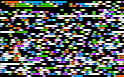
\includegraphics[width=2in]{figures/hidden_vmw.png}
\end{center}
\caption{VMW logo hidden in the executable data.\label{fig:vmw}}
\end{figure}

\begin{figure}[tb]
\begin{center}
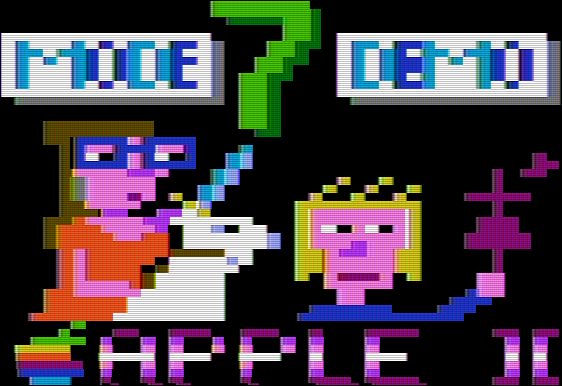
\includegraphics[width=\columnwidth]{figures/mode7_demo_title.png}
\end{center}
\caption{The title screen.\label{fig:title}}
\end{figure}

\begin{figure}[tb]
\begin{center}
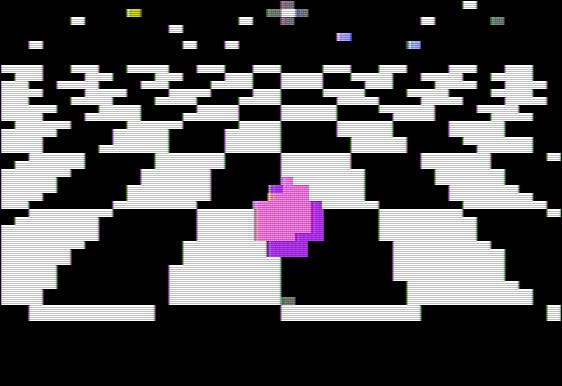
\includegraphics[width=\columnwidth]{figures/m7_screen1.jpg}
\caption{Bouncing ball on infinite checkerboard.\label{fig:ball}}
\end{center}
\end{figure}

\begin{figure}[tb]
\begin{center}
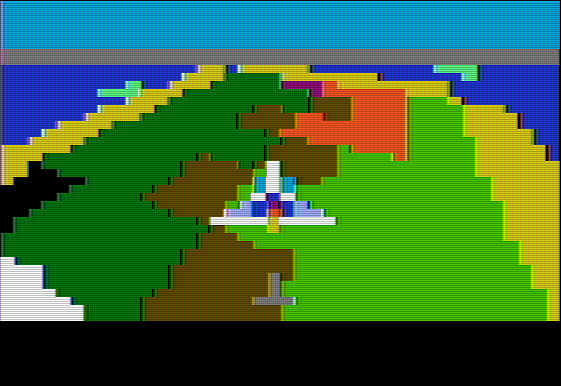
\includegraphics[width=\columnwidth]{figures/m7_screen4.jpg}
\caption{Spaceship flying over an island.\label{fig:tb1}}
\end{center}
\end{figure}

\begin{figure}[tb]
\begin{center}
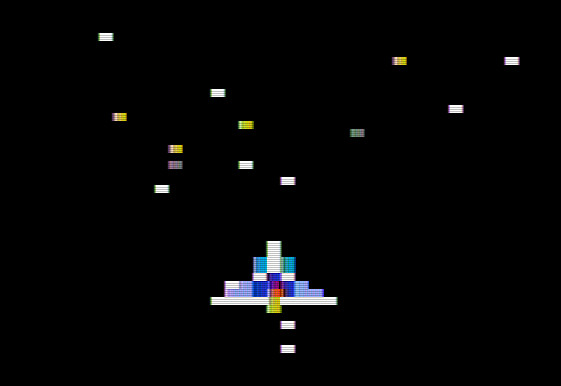
\includegraphics[width=\columnwidth]{figures/m7_screen3.jpg}
\end{center}
\caption{Spaceship with starfield.\label{fig:stars}}
\end{figure}

\begin{figure}[tb]
\begin{center}
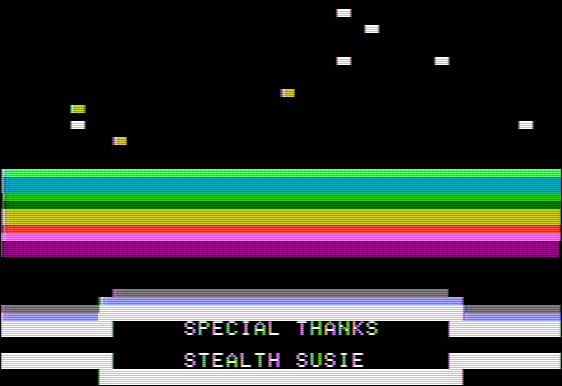
\includegraphics[width=\columnwidth]{figures/m7_screen2.jpg}
\end{center}
\caption{Rasterbars, stars, and credits.  Stealth Susie was a particularly
well-traveled guinea pig.
\label{fig:credits}}
\end{figure}


\section{The Demo}

\subsection{BOOTLOADER}

An Applesoft BASIC ``HELLO'' program loads the binary automatically at bootup.
This does not count towards the executable size, as you could manually BRUN 
the 8k program if you wanted.

To make the loading time slightly more interesting the binary is loaded at
address \$2000 (hi-res page1) and BASIC is nice enough to enable
graphics mode first so you can watch the display get filled with the random
pattern of the compressed image.
This entirely fills the 8k of the display, or would
if we POKEd the right address to turn off
the 4 lines of text on the bottom of the screen.

Upon loading, execution starts at address \$2000

\subsection{DECOMPRESSER}

The binary is encoded with the LZ4 algorithm.
We flip to hi-res Page 2 and decompress there so the user continues to get
a show of random noise.

The 6502 size-optimized LZ4 decompression code was written by qkumba
(Peter Ferrie).
%	http://pferrie.host22.com/misc/appleii.htm
The program and data decompress to around 22k starting at \$4000.
It over-writes parts of DOS3.3, but since we will not be using the disk 
any more this is not an issue.

If you look carefully at the upper left corner of the screen during
decompress you will see my triangular logo, which is supposed to evoke
my VMW initials (see Figure~\ref{fig:vmw}).
To do this I had to put the proper bit pattern at the interleaved
addresses of \$4000, \$4400, \$4800, and \$4C00.  
This turned out to be way more trouble than it was worth.
As an interesting note, the image data at \$4000 is executed as it maps
to (mostly) harmless code.

The demo was optimized to fit in 8k, and this is difficult when your program
is compressed.
Removing instructions sometimes makes the binary {\em larger} as it no longer
compresses as well.
Long runs of values (such as 0 padding) are essentially free.
This mostly turned into an exercise of guess-and-check until everything fit.

\subsection{FADE EFFECT}

The title screen fades in from black.

This is a software hack as the Apple II does not have palette support.
The image is loaded to an off-screen buffer and a lookup table is used to
copy in the faded versions on the fly.

\subsection{TITLE SCREEN}


Once decompression is done, execution continues at address \$4000.
We switch to low-res mode for the rest of the demo.

A title screen is loaded, as seen in Figure~\ref{fig:title}.
The image is run-length encoded (RLE) which is
probably unnecessary when being further LZ4 encoded.
(The LZ4 compression was a late addition to this endeavor).

Why not save some space and just load our demo at \$400 and negate the need
to copy the image in place?
Remember the graphics are 40x48 (shared with the text display region).
It might be easier to think of it as 40x24 characters, with the top / bottom
4-bits of each ASCII character being interpreted as colors for a half-height
block.
If you do the math you will find this takes 960 bytes of space, but the memory
map reserves 1k for this mode.
There are ``holes'' in the address range that are not displayed, and 
various pieces of hardware can use these as scratchpad memory.  
This means just overwriting the whole 1k with data might not work out well
unless you know what you are doing.
To this end the RLE decompression code skips the holes just to be safe.

The title screen has scrolling text at the bottom.
This is nothing fancy, the text is in a buffer off screen and a 40x4 
chunk of RAM is copied in every so many cycles.
You might notice that there is tearing/jitter in the scrolling even
though we are double-buffering the graphics.  
Sadly there is not a reliable cross-platform way to get the VBLANK info 
on Apple II machines, especially the older models.
This is even more noticeable in the recorded video, as the capture card and
movie encoding conspire to make this look worse than things look in person.

\subsection{MOCKINGBOARD MUSIC}

No demo is complete without some exciting background music.
I like chiptune music, especially the kind you can find that is made
for AY-3-8910 based systems.
I gained some expertise during the long wait for my Mockingboard to arrive
by building a Raspberry Pi chiptune player that is essentially the same
hardware.

The song being played is a stripped down and re-arranged version of
``Electric Wave'' from CC'00 by EA (Ilya Abrosimov). 

Most of my sound infrastructure involves YM5 files, a format commonly
used  by ZX Spectrum and ATARI ST users.
These are essentially just AY-3-8910 register dumps taken at 50Hz.  
To play these back just set up the sound card to interrupt 50 times a second
and then write out the 14 register values from that frame.

%   To program the Mockingboard, each AY-3-8910 chip has 14 sound related
%   registers that control the 3 channels.  Each AY chip has a dedicated
%   VIA 6522 parallel I/O chip that handles the I/O.

Writing out the registers quickly enough is a challenge on the Apple II.
For each register you have to do a handshake then set both the register 
number and the value.
It is hard to do this in less than forty 1MHz cycles for each register.
With complex chiptune files (especially those written on an ST with much
faster hardware) it is sometimes not possible to get exact playback
due to the delay.
Further slowdown happens as you want to write both AY chips (the output
is stereo, with one AY on the left and one on the right).
To help with latency on playback we keep track of the last frame written
and only write to the registers that have changed.

%   I have a whole suite of code for manipulating YM sound data, in my
%   vmw-meter git repository.

Our code detects a Mockingboard at startup, we are lazy and only support
finding the card in Slot 4 (which is a fairly typically location).
%   The first step for getting this to work is detecting if a Mockingboard is
%%  there.  This can be in any slot 1-7 on the Apple II, though typically
%   Slot 4 is standard (in this demo we only check slot 4).
The board is initialized, and then one of the 6522 timers is set to
interrupt at 25Hz.
% (it has to be an on-board timer as the default
%   Apple II has no timers).
Why 25Hz and not 50Hz?  At 50Hz with 14 registers you use 700 bytes/s.
So a 2 minute song would take 84k of RAM, much more than is available.
To allow the song to fit in memory (without the fancy circular buffer
decompression utilized in my VMW Chiptune Player music-disk demo) we have
to reduce the size.
First the music is changed so it only needs to be updated at 25Hz.
Then the register data is compressed from 14 bytes to 11 bytes by stripping off
the envelope effects and packing together fields that have unused bits.
In the end the sound quality suffered a bit, but we were able to fit an
acceptably catchy chiptune inside of our 8k payload.

\subsection{MODE7 BACKGROUND}

``Mode7'' is a Super Nintendo (SNES) graphics mode that takes a tiled
background to be transformed by rotation and scaling.
The most common effect was to squash it out to the horizon, giving
a three-dimensional look.
The SNES did these transforms in hardware, but in this demo we implement
them in software.

%  As found on Wikipedia, the transform is of the type
%
%  [x'] = [a b]([x]-[x0])+[x0]
%  [y']   [c d]([y] [y0]) [y0]

Our algorithm is based on code by Martijn van Iersel.
It iterates through each y line on the screen and calculates based on
the camera location: height ({\em spacez}), x and y coordinates 
({\em cx} and {\em cy}) and the {\em angle}.

First calculate the distance
	d = (z*yscale)/(y+horizon)
Then calculate the horizontal scale (distance between points on 
this line)
	h = d/xscale
Then calculate delta x and delta y values
	dx = -sin(angle)*h
	dy = cos(angle)*h
It then calculates the starting offset of the left side of the line in
the tile lookup:
        tilex = cx + (d*cos(angle) - (width/2) * dx;
        tiley = cy + (d*sin(angle) - (width/2) * dy;
Now iterate the inner loop, where we lookup the tile color for each pixel
on the horizontal line.
            putpixel (x, y, tilelookup(tilex,tiley)
            tilex += dx;
            tiley += dy;

{\bf Optimizations}

We managed to take this algorithm and speed it up in the following ways:
	\begin{itemize}
	\item blah 
	\end{itemize}
 
  For our code, we managed to reduce things to a small number of additions
  and subtractions for each pixel on the screen.  Of course the 6502 can't
  do floating point, so we do fixed point math.  We convert as much as we
  can to table lookups that are pre-calculated.  We also make liberal use
  of self-modifying code.

{\bf Fast Multiply:}

  Despite all of this there are still some cases where we have to do a 
  16bit x 16bit = 32bit multiply, something that is *really* slow on 6502,
  around 700 cycles (for a 8.8 x 8.8 fixed point multiply).

  To make this faster we use a method described by Stephen Judd.

  The key to note is that $(a+b)^{2} = a^{2}+2ab+b^{2}$ 
	and $(a-b)^{2}=a^{2}-2ab+b^{2}$
  and if you add them you can simplify to:
	$a\times b =\frac{(a+b)^{2}}{4} - \frac{(a-b)^2}{4}$

  This is you have a table of squares from 0..511 (all 8-bit a+b and a-b
  will fall in this range) then you can convert a multiply into a table
  lookup plus a subtract.

  The downsize is you will need 2kB of squares lookup tables (which can
  be generated at startup).  This reduces the multiply cost to the order
  of 200 to 250 cycles.

  By using the fast multiply and a lot of careful optimization you can
  generate a Mode7 background in 40x40 graphics mode at about 5 frames/second.

  The engine can be parameterized with different tilesets to use, which we
  do to provide both a black+white checkerboard background, as well as the
  island background from the TFV game.

\subsection{BOUNCING BALL ON CHECKERBOARD}

The first scence starts out viewing an infinite checkerboard.
Any demo would be incomplete without some sort of bouncing geometric solid,
in our case a pink sphere.
This was accomplished with 16 sprites:
the sphere was modeled in OpenGL inside of a 20 year old game engine
and screenshots were taken then reduced in keeping with the size and
color limitations.
Similarly the shadow is also just sprites.

The clicking noise on bounce is generated by accessing the speaker port
at address \$C030.
This gives some sound for those viewing the demo without a Mockingboard.

\subsection{TFV SPACESHIP FLYING}


This next scene has a spaceship flying over an island.
The spaceship, water splash, and shadows are all sprites.
They are all drawn in software as the Apple II has no sprite hardware.
The path the ship takes is pre-recorded; this is adapted from the
Talbot Fantasy~7 game engine with the keyboard code replaced by a hard-coded
script of actions to take.

\subsection{STARFIELD}

The spaceship takes to the stars.
This is typical starfield code.
Only 16 stars are modeled, and the movement code re-uses the 
same fast-multiply routine described previously.

The star positions require random number generation, but this is not
fast on the 6502.
Originally we had a 256-byte blob of pre-generated ``random'' values
included in the code.
This wasted space, so now instead we just use our code at address
at \$5000 as if it were a block of random numbers.
This was arbitrarily chosen, and it is not as random as it could be
as seen when the ship enters hyperspace the lower right quadrant has fewer
starts than one could desire.
A simple state machine controls star speed, ship movement, hyperspace,
background color (for the blue flash) and the eventual sequence of sprites
as the ship vanishes into the distance.

\subsection{RASTERBARS/CREDITS}

Once the ship has departed, it is time for the credits as the stars
continue to run.

The text is written to the bottom 4 lines of the screen and appears
to be surrounded by low-res graphics blocks.
Mixed graphics/text would generally not be possible on the Apple II, although
with careful cycle counting and mode switching groups such as FrenchTouch
have achieved this effect.
I was lazy and instead used inverse-mode space characters which appear the same
as white graphics blocks.

The rasterbar effect is not really rasterbars, it's just a colorful assortment
of horizontal lines drawn at a location determined with a sine lookup table.
Horizontal lines can take a surprising amount of time to draw, so this
was optimized using inlining and a few other methods.

The rotating text is done by just rapidly rotating the output string through
the ASCII table, with the clicking effect again by hitting the speaker
at address \$C030.
The list of people to thank ended up being extremely critical to fitting in 8kB,
as unique text strings do not compress well.  
I apologize to everyone whose moniker got compressed beyond recognition,
and I am still not totally happy with the centering of the text.

\section{Obtaining the Code}

More details, disk image, and full source can be found at the website:
\url{http://www.deater.net/weave/vmwprod/mode7_demo/}

%\section{Appendix: Memory Map}


\begin{figure}
\begin{center}
\begin{scriptsize}
\begin{BVerbatim}
 -------------  $ffff
|    ROM/IO   |
 -------------  $c000
|             |
| Uncompressed|
| Code/Data   |
|             |
 -------------  $4000
| Compressed  |
|   Code      |
 -------------  $2000
|   free      |
 -------------  $1c00
|   Scroll    |
|    Data     |
 -------------  $1800
|  Multiply   |
|   Tables    |	
 -------------  $1000
| LORES pg 3  |
 -------------  $0c00
| LORES pg 2  |
 -------------  $0800
| LORES pg 1  |
 -------------  $0400
|free/vectors |
 -------------  $0200
|    stack    |
 -------------  $0100
|   zero pg   |
 -------------  $0000
\end{BVerbatim}
\end{scriptsize}
\end{center}
\caption{Memory Map (not to scale)\label{fig:map}}
\end{figure}



\end{document}
